%This is a Latex file.
\documentclass[12pt]{article}
\usepackage{
	latexsym,
	fancyhdr,
	amsmath,
	amsfonts,
	dsfont,
	amsthm,
	amssymb,
	mathrsfs,
	mathtools
}
\usepackage[margin=0.94in]{geometry}
\usepackage{lastpage} % Required to determine the last page for the footer
\usepackage{tikz}
\usetikzlibrary{arrows.meta}
\usepackage{url, hyperref}

\parindent 0pt

\pagestyle{fancy} \lhead{\sf MTH 411} \chead{\sf Homework \#05}
\rhead{\sf Due: Friday 10/23/2018} \lfoot{} \cfoot{} \rfoot{}

\newcommand{\N}{\mathds{N}}
\newcommand{\Z}{\mathds{Z}}
\renewcommand{\vec}[1]{\overrightarrow{#1}}
\newcommand{\C}{\mathbb{C}}
\newcommand{\R}{\mathbb{R}}
\newcommand{\G}{\mathbb{G}}
\newcommand{\Q}{\mathbb{Q}}
\DeclarePairedDelimiter\abs{\lvert}{\rvert}

\begin{document}
\begin{enumerate}
	\item[7.04] List the elements of the subgroup generated by the given subset: $ \{12,30\} $ of $ \Z_{12} $\\
	As the gcd(12,30) = 6, notice all elements are multiples of the gcd.
	0,6,12,18,24,30
		
	\item[7.05] List the elements of the subgroup generated by the given subset: $ \{12,42\} $ of $ \Z $\\
		$ \cdots,-12-6,0,6,12, \cdots$
	\item[7.06] List the elements of the subgroup generated by the given subset: $ \{18,24,39\} $ of $ \Z $\\
		$ \cdots,-6,-3,0,3,6, \cdots$
	\item[7.07] Compute these products using Fig. 7.11(b).
		\begin{enumerate}
			\item $ (a^2b)a^3 $. Just follow three arcs of $ a $ ending up at $ a^3b $
			\item $ (ab)(a^3b) $. Just follow three arcs of $ a $ and one arc of $ b $ ending up at $ a^2 $
			\item $ b(a^2b) $. Just follow two arcs of $ a $ and one arc of $ b $ ending up at $ a^2 $
 		\end{enumerate}
	\item[7.10] Table for diagraph in Fig. 7.13(c)\\
	\begin{table}[!h]
		\begin{tabular}{l|llllll}
			& e & a & b & c & d & f \\ \hline
			e & e & a & b & c & d & f \\
			a & a & c & f & e & b & d \\
			b & b & d & e & f & a & c \\
			c & c & e & d & a & f & b \\
			d & d & f & c & b & e & a \\
			f & f & b & a & d & c & e
		\end{tabular}
	\end{table}
	
	\item[7.12] Determine whether or not the group corresponding to the Cayley diagraph in Fig. 7.11(b) is commutative.\\
		Not commutative as $ a $ followed by $ b $ gives $ ab $, while $ b $ followed by $ a $ gives $ a^3b $
	\item[7.16] Draw a Cayley digraph for $ \Z_8 $ taking as generating set $ S=\{2,5\} $
	\item[]
		Red = 2, Blue = 5
		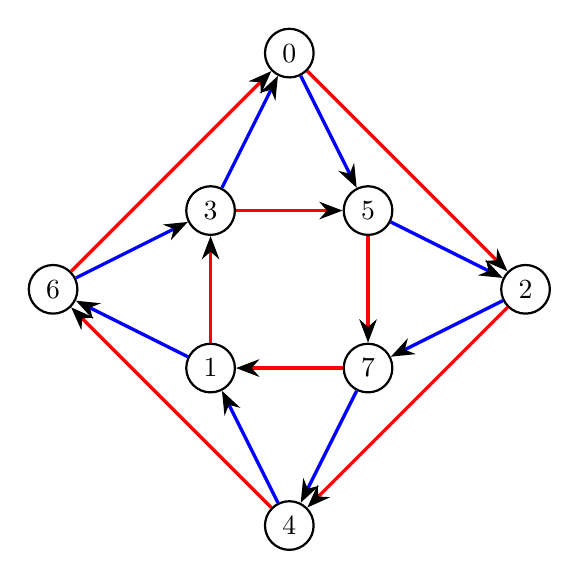
\begin{tikzpicture}
		\begin{scope}[every node/.style={circle,thick,draw}]
			\node(0) at ( 0, 0)   {0};
			\node(1) at (-1,-4)   {1};
			\node(2) at ( 3,-3)   {2};
			\node(3) at (-1,-2)   {3};
			\node(4) at ( 0,-6)   {4};
			\node(5) at ( 1,-2)   {5};
			\node(6) at (-3,-3)   {6};
			\node(7) at ( 1,-4)   {7};
		\end{scope}
		\begin{scope}[>={Stealth[black]}, every edge/.style={draw=red,very thick}]
			\path [->] (0) edge(2);
			\path [->] (2) edge(4);
			\path [->] (4) edge(6);
			\path [->] (6) edge(0);
			
			\path [->] (3) edge(5);
			\path [->] (5) edge(7);
			\path [->] (7) edge(1);
			\path [->] (1) edge(3);
			
		\end{scope}
		
		\begin{scope}[>={Stealth[black]},
		every node/.style={fill=white,circle},
		every edge/.style={draw=blue,very thick}]
			\path [->] (2) edge (7);
			\path [->] (5) edge (2);
			
			\path [->] (0) edge (5);
			\path [->] (3) edge (0);
			
			\path [->] (6) edge (3);
			\path [->] (1) edge (6);
			
			\path [->] (4) edge (1);
			\path [->] (7) edge (4);
			
		\end{scope}
		\end{tikzpicture}
	\item[7.18] Draw digraphs for the two possible structurally different groups of order 4.
	\item[]
	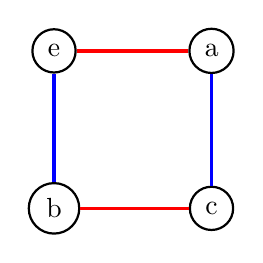
\begin{tikzpicture}
		\begin{scope}[every node/.style={circle,thick,draw}]
		\node(e) at (0,0)    {e};
		\node(b) at (0,-2)   {b};
		\node(a) at (2,0)   {a};
		\node(c) at (2,-2)  {c};
		\end{scope}
		\begin{scope}[>={Stealth[black]},
		every node/.style={fill=white,circle},
		every edge/.style={draw=red,very thick}]
		\path [-] (e) edge (a);
		\path [-] (b) edge (c);
		\end{scope}
		
		\begin{scope}[>={Stealth[black]},
		every node/.style={fill=white,circle},
		every edge/.style={draw=blue,very thick}]
		\path [-] (e) edge (b);
		\path [-] (c) edge (a);
		\end{scope}
	\end{tikzpicture}
	
	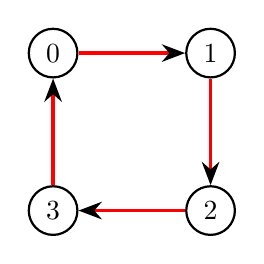
\begin{tikzpicture}
		\begin{scope}[every node/.style={circle,thick,draw}]
		\node(0) at (0,0)    {0};
		\node(1) at (2,0)    {1};
		\node(2) at (2,-2)   {2};
		\node(3) at (0,-2)   {3};
		\end{scope}
		\begin{scope}[>={Stealth[black]},
		every node/.style={fill=white,circle},
		every edge/.style={draw=red,very thick}]
		\path [->] (0) edge (1);
		\path [->] (1) edge (2);
		\path [->] (2) edge (3);
		\path [->] (3) edge (0);
		\end{scope}
	\end{tikzpicture}
	
	\item[]
	$\sigma = \begin{pmatrix}
	1 & 2 & 3 & 4 & 5 & 6 \\
	3 & 1 & 4 & 5 & 6 & 2 
	\end{pmatrix}  $
	$\tau = \begin{pmatrix}
	1 & 2 & 3 & 4 & 5 & 6 \\
	2 & 4 & 1 & 3 & 6 & 5 
	\end{pmatrix}  $
	$\mu = \begin{pmatrix}
	1 & 2 & 3 & 4 & 5 & 6 \\
	5 & 2 & 4 & 3 & 1 & 6 
	\end{pmatrix}  $
	
	\item[8.02] Compute the indicated product: $ \tau^2\sigma $
		\[\begin{pmatrix}
		1 & 2 & 3 & 4 & 5 & 6 \\
		2 & 4 & 1 & 5 & 6 & 3 
		\end{pmatrix}  \]
	\item[8.04] Compute the indicated product: $ \sigma^{-2}\tau $ 
			\[\begin{pmatrix}
			1 & 2 & 3 & 4 & 5 & 6 \\
			5 & 1 & 6 & 2 & 4 & 3 
			\end{pmatrix}  \]
	\item[8.08] Compute the expression shown for $ \sigma^{100} $
			\[\sigma^{100}=(\sigma^6)^{16}\sigma^4=\sigma^4 =
			\begin{pmatrix}
			1 & 2 & 3 & 4 & 5 & 6 \\
			2 & 4 & 1 & 5 & 6 & 3 
			\end{pmatrix}  \]
	\item[8.12] Find the orbit of 1 under the permutation defined earlier: $ \tau $
		\[\{1,2,3,4\}\]
	\item[8.18a] Find the cyclic subgroups $ \langle \rho_1\rangle, \langle \rho_2\rangle $, and  $\langle \mu_1\rangle $  of $ S_3 $
		\[\langle \rho_1 \rangle = \langle \rho_2 \rangle = \{\rho_0,\rho_1,\rho_2\}\] \[\langle \mu_1 \rangle = \{\rho_0,\mu_1\} \]
	\item[8.18b] Find \textit{all} subgroups, proper and improper, of $ S_3 $ and give the subgroup diagram for them.
	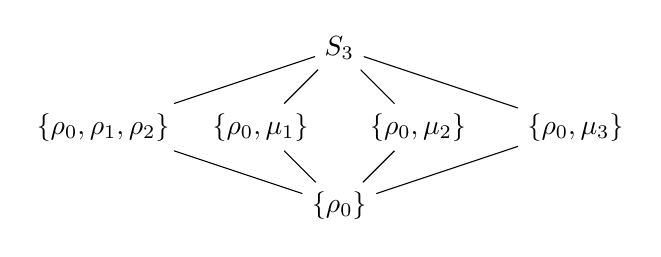
\begin{tikzpicture}
		\begin{scope}[]
		\node(S) at (0,0)    {$ S_3 $};
		\node(1) at (-3,-1)    {$ \{\rho_0,\rho_1,\rho_2 \} $};
		\node(2) at (-1,-1)   {$ \{\rho_0,\mu_1\} $};
		\node(3) at (1,-1)   {$ \{\rho_0,\mu_2 \} $};
		\node(4) at (3,-1)   {$ \{\rho_0,\mu_3 \} $};
		\node(5) at (0,-2)   {$ \{\rho_0\} $};
		\end{scope}
		\begin{scope}[]
		\path [-] (S) edge (1);
		\path [-] (S) edge (2);
		\path [-] (S) edge (3);
		\path [-] (S) edge (4);
		\path [-] (1) edge (5);
		\path [-] (2) edge (5);
		\path [-] (3) edge (5);
		\path [-] (4) edge (5);
		\end{scope}
	\end{tikzpicture}
	\item[8.20] Give the multiplication table for the cyclic subgroup of $ S_5 $ generated by 
		\[\rho = \begin{pmatrix}
		1 & 2 & 3 & 4 & 5 & 6 \\
		3 & 1 & 4 & 5 & 6 & 2 
		\end{pmatrix} \]
	There will be six elements. Let them be $ \rho, \rho^2, \rho^3, \rho^4, \rho^5,$ and $ \rho^0 = \rho^6 $. Is this group isomorphic to $ S_3 $?\\
	Not isomorphic, as the group is abelian, while $ S_3 $ is not abelian.
	\item[8.28] A \textit{permutation} of a set $ S $ is a one-to-one map from $ S $ to $ S $
		A \textit{permutation} of a set S is a one-to-one map of $S$ onto $S$.
	\item[8.29]The \textit{left regular representation} of a group $ G $ is the map of $ G $ into $ S_G $ whose value at $ g\in G $ is the permutation of $ G $ that carries each $ x\in G $ into $ gx $\\
	Correct as stated.
	\item[8.36] Show by an example that every proper subgroup of a nonabelian group may be abelian.\\
	$ S_3 $ is a good example. $ S_3 $ is nonabelian, yet all of its proper subgroups are abelian.
		
	\item[8.38] Indicate schematically a Cayley digraph for $ D_n $ using a generating set consisting of a rotation through $ 2\pi/n $ radians and a reflection.\\
	Let $ R $, red, = rotation and $ F $, green, = flip.\\
		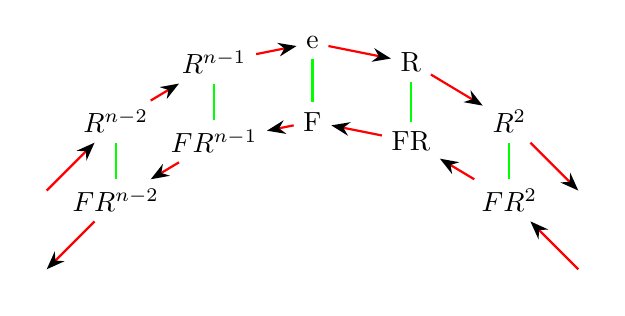
\begin{tikzpicture}
			\begin{scope}[]
				\node(e)   at (0,0)   		 {e};
				\node(R)   at (1.25,-.25)    {R};
				\node(R2)  at (2.5,-1)  	 {$ R^2 $};
				\node(R3)  at (3.5,-2)  	 {};
				\node(Rn1) at (-1.25,-.25)   {$ R^{n-1} $};
				\node(Rn2) at (-2.5,-1) 	 {$ R^{n-2} $};
				\node(Rn3) at (-3.5,-2) 	 {};
				
				\node(F)   at (0,-1)    	{F};
				\node(FR)   at (1.25,-1.25)   {FR};
				\node(FR2)  at (2.5,-2)  	{$ FR^2 $};
				\node(FR3)  at (3.5,-3)  	 {};
				\node(FRn1) at (-1.25,-1.25)  {$ FR^{n-1} $};
				\node(FRn2) at (-2.5,-2)  	{$ FR^{n-2} $};
				\node(FRn3) at (-3.5,-3) 	 {};
			\end{scope}
			\begin{scope}[>={Stealth[black]},
			every edge/.style={draw=red,thick}]
				\path [->] (Rn3) edge (Rn2);
				\path [->] (Rn2) edge (Rn1);
				\path [->] (Rn1) edge (e);
				\path [->] (e) edge (R);
				\path [->] (R) edge (R2);
				\path [->] (R2) edge (R3);
				
				\path [<-] (FRn3) edge (FRn2);
				\path [<-] (FRn2) edge (FRn1);
				\path [<-] (FRn1) edge (F);
				\path [<-] (F) edge (FR);
				\path [<-] (FR) edge (FR2);
				\path [<-] (FR2) edge (FR3);
			\end{scope}
			
			\begin{scope}[>={Stealth[black]},
			every edge/.style={draw=green,thick}]
				\path [-] (Rn2) edge (FRn2);
				\path [-] (Rn1) edge (FRn1);
				\path [-] (e) edge (F);
				\path [-] (R) edge (FR);
				\path [-] (R2) edge (FR2);
			\end{scope}
		\end{tikzpicture}

	\item[8.46] Show that $ S_n $ is a nonabelian group for $ n \geq  3$.

	\item[8.48] Let $ a,b \in A $ and $ \sigma \in S_a $. Show that if $ \mathcal{O}_{a,\sigma} $ and $ \mathcal{O}_{b,\sigma} $ have an element in common, then $ \mathcal{O}_{a,\sigma}  = \mathcal{O}_{b,\sigma}$.

	\item[8.50] Show that for $ \sigma \in S_a, \langle \sigma \rangle $ is transitive on A if and only if $ \mathcal{O}_{a,\sigma}=A $ for some $ a\in A $
	
\end{enumerate}
\end{document}
